Cuanto disponemos de varios resultados obtenidos de distintas fuentes biométricas para poder evaluar como afectan cada uno de los resultados en la decisión desarrollaremos un sistema de fusión de caracterísicas biométricas.

\section{Datos de entrada}
Para este ejercicio disponemos de ficheros con texto plano cuya última columna nos indica si el dato es un cliente o un impostor y en las columnas anteriores tenemos los resultados de los distintos sistemas biométricos. En este caso únicamente 2 scores.

\section{Desarrollo realizado}
\subsection{Tratamiento de los datos de entrada}
En primer lugar desarrollamos un pequeño script bash, que separe los scores de los clientes y de los impostores y se quede con una subsección de los mismos, para acelerar los cálculos. En caso de llevar este sistema a producción el número de elementos en el subconjunto deberá se el total de los elementos disponibles.\par

\subsection{Fusión de scores}
Con los datos ya preparados realizamos un script en python que lea estos datos y calcule el peso para cada score de modo que se minimice el área bajo la curva ROC.\par
En el listado de código \ref{fusion:sol} podemos ver las opciones para lanzar el script.\par


\begin{lstlisting}[language=python,label=fusion:uso, caption=PCA cuado n es menor d]

$ python fusion.py --help                         
usage: fusion.py [-h] [-tr TR] [-te TE] [-p]

Fuse some scores
optional arguments:
  -h, --help          show this help message and exit
  -tr TR, --train TR  Scores for train data
  -te TE, --test TE   Scores for test data
  -p, --plot          Make plot
\end{lstlisting}


\section{Resultados}

A continuación, en el segmento de código \ref{fusion:sol}, vemos los resultados de la fusión de los dos scores de modo que minimicen el área bajo la curva ROC. Y en la figura \ref{fig:fusion} vemos como se distribuyen los dos scores tanto en entrenamiento como en pruebas.\par

\begin{lstlisting}[language=python,label=fusion:sol, caption=PCA cuado n es menor d]
$ python fusion.py -tr ../data/fusion/train_small -te ../data/fusion/test_small -p
El valor máximo del área bajo la curva ROC= 1.423700 
Con los pesos:
  [ 0.60, 0.40 ]
\end{lstlisting}

\begin{figure}[h!]
  \centering
      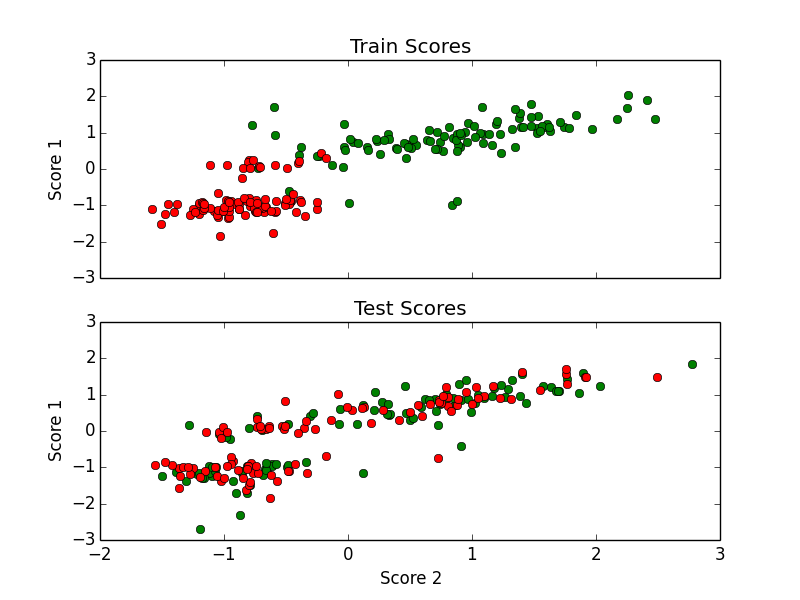
\includegraphics[width=0.7\textwidth]{../fusion/fusion.png}
  \caption{ Scores en train y en test}
  \label{fig:fusion}
\end{figure} 
